\section{Technical preliminaries}
\label{preliminaries}
In this section we briefly review the notions of abstraction and over-approximation of system.
Let $M$ be a system model and $S$ be its state space (in Section ??? we give a specific formalism in which our systems are modeled).
A \emph{trace} $\straj$ of $M$ is an infinite sequence of states produced by $M$: $\straj \in S^\omega$.
The \emph{behavior} $\beh(M) \subset S^\omega$ of $M$ is then the set of all its possible traces.

Let $AP$ be a set of atomic propositions and $\phi$ be an ACTL$^*$ formula over $AP$ [???].
ACTL$^*$ is the fragment of CTL$^*$ with only the universal quantifier (``for every path'').
The set of $M$ traces that satisfy $\phi$ is denoted by $\beh(\phi)$. 
It holds by definition that if $M$ satisfies $\phi$, then $\beh(M) \subset \beh(\phi)$.
We write this as $M \models \phi$.
A model checker takes $M$ and $\phi$ as inputs and either returns SAT, meaning that $M \models \phi$, or returns a \emph{counter-example}, which is a trace $\straj \in \beh(M) \setminus \beh(\phi)$.

An \emph{abstraction function} $\absfun: S \rightarrow S'$ maps the states of $M$ to new \emph{abstract} states.
We extend it to traces and sets of traces in a natural manner: $\absfun(\straj) =  \absfun(s_0)\absfun(s_1)\ldots$ for $\straj = s_0 s_1\ldots \in S^\omega$,
and $\absfun(W) = \cup_{\straj \in W}\absfun(\straj)$ for any $W \subset S^\omega$.
The abstraction function is total (i.e. defined for every $s \in S$) and is such that
\[R(\beh(M)) \subset \beh(M') \]
where $\absfun(W) = \cup_{\straj \in W} \absfun(\straj)$.
Abstraction is used to reduce the size of the state space ($|S'| < |S|$), so that model checking becomes feasible on the new model $M'$ with state space $S'$, while preserving behavior.
Indeed, if $R(\beh(M)) \subset  \beh(M') $ and $\beh(M') \subset \beh(\phi)$, then it holds that $\beh(M) \subset \beh(\phi)$ and so $M \models \phi$ (here we omit certain technicalities relating to the appropriateness of the abstraction function $\absfun$ to $\phi$. The reader is referred to [Section 3, Clarke JACM] for a good overview).

A \emph{closed loop requirement} is an ACTL$^*$ formula $\formula_C$ of the form $\formula_C :=\formula_E \implies \formula_D$ in which $\formula_E$ describes the open-loop environment behavior that the device encounters, and $\formula_D$ is the closed-loop behavior that the device should achieve. 

A \emph{closed loop requirement} is an ACTL$^*$ formula of the form$\formula_E\Rightarrow \formula_C$ where $\formula_E$ is a specification on the environment model and $\formula_C$ is a specification on the closed-loop model.
For example, 
\[\textrm{AtrialSense} \implies \eventually ((\textrm{VentricularSense } ||  \textrm{ VentricularPace }) \land  t \leq 500)\]
 expresses that if the heart displays electrical activity in the atrium (an `atrial sense'), then there should be electrical activity in the ventricles within 500ms (either naturally or as a result of a pacing event).

\subsubsection{Spurious vs physiologically valid counter-examples}
Suppose a model checker is run on an abstract model $M'$ obtained by abstracting $M$ using some abstraction function $R$.
If the checking returns a counter example $\straj \in \beh(M')$, two cases are possible:
either $R^{-1}(x) \in \beh(M)$, or not.
In the first case, there is no ambiguity: this is a valid counter-example.
In the second case $R^{-1}(x) \notin \beh(M)$, the trace $\straj$ is usually discarded as being spurious.
This makes sense if the model $M$ is taken to be the ground truth: i.e. anything not generated by $M$ is not valid behavior. 
However, when modeling the environment for closed-loop verification, $M$ is only one of many models, none of which is ground truth. 
That is, it is recognized that there exists physiologically meaningful behavior not captured by any of the models. 
In this case, we use abstraction functions not only to reduce the size of the state space, but mainly to \emph{introduce, in a systematic manner, physiologically meaningful behavior}. 
Thus a counter-example $\straj$, while not producable by any of the initial models, may still be a valid example.

\begin{figure}[!t]
		\centering
		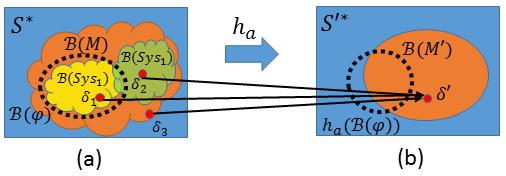
\includegraphics[width=0.8\textwidth]{figs/distinction.png}
		%\vspace{-5pt}
		\caption{\small Two models such that $Sys1$ and $Sys2$ are combined into $M$, which is further abstracted into $M'$ using rule $h_a$. By model checking $M'$ against property $\formula$ we have $M'\not\models\formula$ and $\delta$ is returned as counter-example. $\delta$ corresponds to 3 different behaviors in the original behavior space: $\delta_1$ satisfies $\formula$ and is produced by $Sys1$, $\delta_2$ falsifies $\formula$ and is produced by $Sys2$, and $\delta_3$ unsatisfied and invalid}
		  %\vspace{-15pt}
		\label{fig:ambiguity}
\end{figure}

